\Chapter{Témaköri felvezetés}

\Section{A darts bemutatása}

A darts Angliából származó játék és sport, melynek a lényege hogy apró nyilakkal eltaláljuk a céltábla különböző pont értékű szektorait. A táblán összesen 20 plusz 1 szektor található meg, a 20 szektor értéke értelemszerűen 1-től 20-ig határolható be, de táblán belül megtalálható még két gyűrű is, a belső gyűrű amelyet, ha eltálunk akkor az adott szektor értékének a háromszorosát érjük el egy dobással, a külső gyűrű eltalálásával pedig a dobás szektor értékének kétszerese. A plusz 1 szektor pedig a tábla közepén megtalálható kis kör amelyet a sportban Bulseye-nak, vagy röviden csak Bull-nak nevezünk. Ezt a kört két részre osztjuk fel, a külső Bull értéke 25, a belsőé pedig 50. 
Egy mérkőzést szettekre, a szetteket legekre, a legeket pedig körökre osztjuk fel. Egy körben minden játékosnak 3 nyíl áll a rendelkezésére és ebből a 3 dobásból a maximálisan megszerezhető pontok száma pedig 180, ezt a tripla 20-as szektor háromszori eltalálásával tudjuk elérni. Egy legben minden játékos 501 pontról kezd, ebből kerül kivonásra minden kör után az adott körben dobott pontszámuk. Egy leg megnyeréséhez a 0 pont pontos elérése szükséges, ráadásul úgy, hogy az utolsó eldobott nyílnak dupla szektort kell eltalálnia. Amint egy játékos olyan pontszámot ér el, amely pontosan elérhető 3 dobásból, úgy hogy az utolsó nyilát dupla szektorba dobja, akkor azt kiszállónak nevezzük. A legmagasabb pontszám amiről ki lehet szállni, a 170, amit a tripla 20-as szektor kétszeres és végezetül a belső Bull egyszeres eltalálásával (mivel az dupla 25-nek számít) érhető el. Egy leg legkevesebb 9 nyílból nyerhető meg, ennek a megdobására több féle kombináció is létezik. Egy szett megnyeréséhez általában 3 leg megnyerése szükséges egy játékos számára, azonban a profi dartsban ritkák azok a versenyek amelyeket szettekre játszanak, a nagyobb tornák közül csak a Világbajnokság és a World Grand Prix ilyen. Ezekből adódóan egy mérkőzés megnyeréséhez a szabályzatban meghatározott számú legek vagy szettek száma szükséges. Ezen felsorolt szabályok egy általános mérkőzés típusra vonatkoznak, a játéknak vannak még különbféle változatai amelyekre más szabályok vonatkoznak, ezekre még a későbbiekben ki fogok térni.


\Section{A darts matematikai modellje}

Az alábbiakban, egy matematikai modellben szeretném szemléltetni azokat a lépéseket, amelyek egy leg megnyeréséhez szükségesek egy klasszikus típusú mérkőzésen:
\begin{enumerate}
\item Játék kezdete:
\begin{itemize}
\item A játékosok kisorsolják, hogy ki kezdi a játékot.
\item Minden játékosnak 301/501/701 pontja van kezdéskor.
\end{itemize}
\item Dobás menete:
\begin{itemize}
\item A játékosok felváltva dobnak három nyilat.
\item A dobás eredménye (pontértékek) levonódnak a játékos aktuális pontszámból.
\end{itemize}
\item Pontszámítás:
\begin{itemize}
\item Az alap pontszámítás szerint minden eltalált szektor pontértéke levonódik a játékos pontszámából.
\item Amikor a játékos eltalálja a dupla szektorok valamelyikét, akkor az eltalált pontszám duplájával, ha a tripla szektor valamelyikét, akkor pedig a triplájával csökken a játékos pontszáma.
\item Amennyiben a játékos túllépi a 501 pontot, akkor az adott dobás nem számít, és a játékos visszatér az előző pontszámához.
\end{itemize}
\item Kiszállás:
\begin{itemize}
\item A játékosnak pontosan 0 pontot kell elérnie a kiszálláshoz.
\item A kiszálló csak akkor érvényes, ha a meghatározott szabályok alapján történik, vagyis ha csak duplával lehet kiszállni, akkor az utolsó eltalált szektornak duplának kell lennie, ha viszont nincs ilyen szabály akkor az utolsó eltalált szektor lehet szimpla, dupla és akár tripla is.
\end{itemize}
\item Játék vége:
\begin{itemize}
\item A játék lezárásához valamelyik játékosnak ki kell szállnia.
\item Amelyik játékos először kiszáll az győz.
\end{itemize}
\end{enumerate}
\begin{figure}[h]
\centering
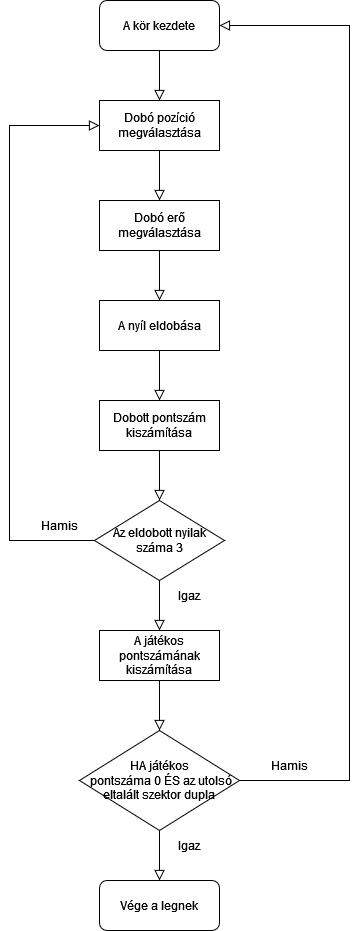
\includegraphics[scale=0.3]{images/darts_flowchart.drawio}
\caption{Darts folyamatábrája}
\label{fig:cimer}
\end{figure}


\Section{Felhasznált technológiák - Frontend}
\subsection{Angular}
Az Angular egy nyílt forráskódú, TypeScript nyelven írt JavaScript keretrendszer. Az Angular mint keretrendszer számottevő előnnyel rendelkezik, miközben szabványos struktúrát biztosít a fejlesztők számára, amellyel dolgozhatnak. Lehetővé teszi a felhasználók számára, hogy nagyméretű alkalmazásokat hozzanak létre karbantartható módon. A használata sok előnnyel jár, mivel a keretrendszer alapja, a JavaScript nagyon sok helyen előfordul manapság, viszont önmagában a JavaScript nem teljesen ideális olyan oldalak fejlesztésére, amelyek modularitást, tesztelhetőséget és fejlesztői produktivitást igényelnek. Az egyéb JavaScript alapú keretrendszerek mellett az Angular ilyen és ehhez hasonló problémákra nyújt megoldást.

Az Angular keretrendszert az alkalmzásom Frontend részének a fejlesztése közben használtam, aminek a segítségével nagyon sok fejlesztési lehetőségem nyílt és a komponens alapú architektúrájának köszönhetően az alkalmazásom dinamikus és átláthatóbb lett.
\cite{Angular}
\subsection{HTML és CSS}
A HTML és CSS használata véleményem szerint nem szorul különösebb indoklásra és ajánlásra. Ezen két nyelvnek a használata elengedhetetlen manapság a webfejlesztők számárá, hiszen a modern web-es alkalmazások legnagyobb része már ezeken alapul. A HTML a címkék és törések rendszerének segítségével határozza meg a böngésző számára megjeleníteni kívánt tartalmat. A CSS ezen tartalmaknak a megjelenítését határozza meg amire számos opciónk van (pl.: színek, méretek, pozíciók, betűtípusok, stb.).Ez a két nyelv együttesen segít egyszerű, szövegekből, képekből és hiperhivatkozásokból álló weboldalak létrehozásában.
https://www.nobledesktop.com/learn/html-css/why-learn-html-css
\Section{Felhasznált technológiák - Backend}
\subsection{Node.JS - Express}
 A Node (vagy hivatalosabban Node.js) egy nyílt forráskódú, platformok közötti futtatókörnyezet, amely lehetővé teszi a fejlesztők számára, hogy mindenféle szerveroldali eszközt és alkalmazást készítsenek JavaScriptben. A futtatási időt a böngésző környezetén kívüli használatra szánják (azaz közvetlenül egy számítógépen vagy szerver operációs rendszeren való futtatásra). Mint ilyen, a környezet elhagyja a böngésző-specifikus JavaScript API-kat, és támogatja a hagyományosabb operációs rendszer API-kat, beleértve a HTTP és a fájlrendszer könyvtárakat.
 
\begin{itemize}
\item A Node-ot úgy tervezték, hogy optimalizálja a webes alkalmazások áteresztőképességét és skálázhatóságát, és jó megoldás számos gyakori webes fejlesztési problémára (pl. valós idejű webes alkalmazások).
\item A kódot "egyszerű régi JavaScriptben" írja, ami azt jelenti, hogy kevesebb időt kell a nyelvek közötti "kontextusváltással" foglalkozni, amikor kliens- és szerveroldali kódot egyaránt ír.
\item A JavaScript egy viszonylag új programozási nyelv, és a nyelvtervezésben elért fejlesztések előnyeit élvezheti más hagyományos webszerver-nyelvekhez (pl. Python, PHP stb.) képest. Sok más új és népszerű nyelv fordít/konvertál JavaScriptbe, így a TypeScript, CoffeeScript, ClojureScript, Scala, LiveScript stb. is használható.
\item  A node csomagkezelő (npm) több százezer újrafelhasználható csomaghoz biztosít hozzáférést. Emellett a legjobb függőségi feloldással rendelkezik, és a build toolchain nagy részét is automatizálhatja.
\item Elérhető Microsoft Windows, macOS, Linux, Solaris, FreeBSD, OpenBSD, WebOS és NonStop OS rendszereken. Továbbá számos webtárhely-szolgáltató jól támogatja, amelyek gyakran speciális infrastruktúrát és dokumentációt biztosítanak a Node-oldalak hosztolásához.
\end{itemize}

A Node.js segítségével egyszerű webkiszolgálót hozhat létre a Node HTTP csomag segítségével.


Az Express a legnépszerűbb Node webes keretrendszer, és számos más népszerű Node webes keretrendszer alapkönyvtára. Mechanizmusokat biztosít a következőkhöz:

\begin{itemize}
\item Kezelőprogramok írása különböző HTTP igékkel rendelkező kérésekhez különböző URL-útvonalakon.
\item Integrált a "view" renderelő motorokkal azért, hogy válaszokat generáljanak az adatok sablonokba illesztésével.
\item Általános webalkalmazási beállítások beállítása, például a csatlakozáshoz használandó port és a válasz rendereléséhez használt sablonok helye.
\item További kérésfeldolgozó "middleware" hozzáadása a kéréskezelő csővezeték bármely pontján.
\end{itemize}


Míg az Express maga meglehetősen minimalista, a fejlesztők kompatibilis middleware-csomagokat hoztak létre szinte bármilyen webfejlesztési probléma megoldására. Vannak könyvtárak a cookie-k, munkamenetek, felhasználói bejelentkezések, URL-paraméterek, POST-adatok, biztonsági fejlécek és még sok más adat kezelésére.


A Node.js és az Express ideális választás olyan alkalmazások esetében amelyeknek a Frontend-je Angular, ezért is esett erre a választásom. Mivel mind a Node.js, mind az Angular JavaScript alapú keretrendszer, ezért kényelmes a közös használatuk és a kódbázis is könnyebben használható fel újra.  Az Angular és a Node.js közötti adatkommunikáció természetes, hiszen mindkettő aszinkron és eseményvezérelt megközelítést alkalmaz. Az Express lehetővé teszi az egyszerű API-k kialakítását, amelyek könnyen integrálhatók az Angular frontendjébe, például a HTTP kérések kezelésére. Node.js és Express együtt rugalmas megoldást nyújtanak a háttérlogika megvalósítására. A backend oldalon a különböző metódusok, hívások könnyen tesztelhetőek, egyszerű struktúrával rendelkeznek, így logikailag könnyebb volt az alkalmazás megtervezése és felépítése. Az Angular és a Node.js - Express kombinációja tehát egy erőteljes és kényelmes megoldást nyújt a teljes verziós JavaScript alkalmazások fejlesztéséhez. 
ÖSSZEHASONLÍTÁS
\subsection{MongoDB}
A MongoDB, a legnépszerűbb NoSQL adatbázis, egy nyílt forráskódú dokumentumorientált adatbázis. A "NoSQL" kifejezés jelentése "nem relációs". Ez azt jelenti, hogy a MongoDB nem a táblázatszerű relációs adatbázis-struktúrán alapul, hanem egy teljesen más mechanizmust biztosít az adatok tárolására és visszakeresésére. Ezt a tárolási formátumot BSON-nak ( a JSON formátumhoz hasonló) nevezik. Ha az adatbázis egyetlen szerveren fut, akkor eléri a skálázási határt. A NoSQL-adatbázisok jobban skálázhatók és jobb teljesítményt nyújtanak. A MongoDB egy ilyen NoSQL adatbázis, amely újabb és újabb szerverek hozzáadásával skálázódik, és rugalmas dokumentummodelljével növeli a termelékenységet. A MongoDB indexelést használ a hatékony keresés érdekében, így a teljes adatmennyiség rövid idő alatt feldolgozható. A MongoDB növeli az adatok rendelkezésre állását az adatok különböző szervereken lévő többszörös másolataival. A redundancia biztosításával megvédi az adatbázist a hardverhibáktól. Ha egy szerver leáll, az adatok könnyen lekérdezhetők a többi aktív szerverről, amelyeken szintén tárolták az adatokat. A MongoDB az egyszerűsége miatt jelentősen megkönnyítette az alkalmazás fejlesztését. Különösképpen a mongoose-t szeretném kiemelni, amelynek a segítségével könnyebb volt az adatmodellek felépítése, a beépített metódusaival pedig egyszerűen és röviden elvégezhető volt minden adatbázis művelet. 
(https://www.geeksforgeeks.org/mongodb-an-introduction/)

